\documentclass[a4paper,11pt]{article}

\usepackage[a4paper,margin=1in]{geometry}
\usepackage[utf8]{inputenc}
\usepackage{amsmath}
\usepackage{amssymb}
\usepackage{amsthm}
\usepackage{booktabs}
\usepackage[small]{caption}
\usepackage{cite}
\usepackage{colortbl}
\usepackage{enumitem}
\usepackage{framed}
\usepackage{graphicx}
\usepackage{multirow}
\usepackage{microtype}
\usepackage[dvipsnames]{xcolor}
\usepackage[unicode]{hyperref}
\usepackage{amsfonts}
\usepackage{algorithm}
\usepackage{algpseudocode}
\usepackage{bm}
\usepackage{mathtools}
\usepackage{subcaption}

\usepackage{listings} % replace with nice syntax hl

\bibliographystyle{plainurl}

\setlength{\OuterFrameSep}{0.3ex}
\setlength{\FrameSep}{1.5ex}

\newcommand{\myaff}[1]{\,$\cdot$\, {\small #1}\par\smallskip}
\newcommand{\fakeparagraph}[2]{\par\noindent\textbf{#1}\hspace{1em}#2}

\usepackage{thm-restate}
\usepackage{cite}

% Problem definition environment
\newfloat{problemdef}{htbp}{loa}
\floatname{problemdef}{Problem}
\newcommand{\problemcaptionkludge}{\rule[-.3\baselineskip]{0pt}{\baselineskip}}

\theoremstyle{plain}
\newtheorem{theorem}{Theorem}[section]
\newtheorem{lemma}[theorem]{Lemma}
\newtheorem{corollary}[theorem]{Corollary}
\newtheorem{observation}[theorem]{Observation}
\theoremstyle{definition}
\newtheorem{definition}[theorem]{Definition}
\newtheorem{example}[theorem]{Example}
\theoremstyle{remark}
\newtheorem*{remark}{Remark}
\newtheorem{openquestion}[theorem]{Open question}

\newcommand{\tcode}[1]{\texttt{#1}}
\newcommand{\tperm}[1]{\texttt{#1}}
\newcommand{\tsub}[1]{\textsubscript{#1}}

% Well-parenthesized commands
\newcommand{\set}[1]{\ensuremath{\left\{#1\right\}}}

\newenvironment{myabstract}
{\list{}{\listparindent 1.5em%
        \itemindent    \listparindent
        \leftmargin    0cm
        \rightmargin   0cm
        \parsep        0pt}%
    \item\relax}
{\endlist}

\newenvironment{mycover}
{\list{}{\listparindent 0pt
        \itemindent    \listparindent
        \leftmargin    0cm
        \rightmargin   0cm
        \parsep        0pt}%
    \raggedright
    \item\relax}
{\endlist}

\begin{document}

\begin{mycover}
{\huge\bfseries\boldmath Tree Borrows\par}
\bigskip
\bigskip
\bigskip


Author: \textbf{Neven Villani}
\myaff{ENS Paris-Saclay}

~\newline

Advisor: \textbf{Derek Dreyer}
\myaff{MPI for Software Systems}


Advisor: \textbf{Ralf Jung}
\myaff{ETH Zürich}


\end{mycover}
\medskip

\begin{myabstract}
\fakeparagraph{Abstract.}
\end{myabstract}
\medskip


\section{Introduction}

While the purpose of type systems and typing information in programs is usually
presented as primarily a matter of security (strict type systems can rule out
at compilation-time a number of bugs), they also enable compilers to generate
more efficient code in both space and time. Languages with strict compile-time
type systems can avoid the need for typing metadata at runtime, have fewer
bounds checks for memory accesses, or even in the case of Rust eliminate the
need for a runtime garbage collector entirely.

In Rust the type system includes aliasing information (mutability and uniqueness),
which is to be used not only for safety guarantees, but also to improve
performance and enable optimizations that are only valid under certain aliasing
guarantees.
We aim to define formally what these aliasing guarantees are for Rust, as
well as show how to check them and use them in proving the validity of compiler
optimizations.

\subsection{Motivating example}

As a first concrete example, consider the following function:
\begin{lstlisting}
fn example1(x: &mut u64, y: &mut u64) -> u64 {
     let xval = *x; // First read of *x
     *y = xval + 1;
     let xval = *x; // Second (redundant ?) read of *x
     return xval;
}
\end{lstlisting}

Because mutable references in Rust are required to be unique, \tcode{x} and
\tcode{y} must point to disjoint regions of memory. In particular the
instruction \tcode{*y = xval + 1} constitutes a write to \tcode{y}, but it
cannot affect the memory covered by \tcode{x}: the value \tcode{*x} is unaffected
and thus the second read of \tcode{*x} is redundant. This function can be
optimized to perform one fewer operation by deleting the second line on which
\tcode{*x} is read, without modifying behavior.

Unfortunately there is a huge gap in the proof above: we have not specified
by whom, in what contexts or in which manner mutable references are ``required''
to be unique. This is the purpose of Tree Borrows.

Indeed there exists in Rust the \tcode{unsafe} keywords which
allows the programmer to bypass certain compiler checks by extending their
available instruction set: among other things the \tcode{unsafe} keyword allows
dereferencing raw pointers in the following manner:
\begin{lstlisting}
fn context1() {
    let mut data = 42u64;
    let data_ptr = &mut data as *mut u64;
    let x: &mut u64 = unsafe { &mut *data_ptr };
    let y: &mut u64 = unsafe { &mut *data_ptr };
    let result = example1(x, y);
    assert!(result == 43);
}
\end{lstlisting}
Here we use \tcode{unsafe} instructions to obtain two mutable references
to the same location, and we pass both of them to \tcode{example1}.
While in this context the original version of \tcode{example1} will return
\tcode{43}, the optimized version will instead return \tcode{42}.

The optimization shown here is thus not unconditionally valid: violating the
unicity requirement of mutable references has enabled us to create a program
in which the optimization does not preserve behavior.

However we want this optimization to be valid, on the grounds of \tcode{context1}
being a ``bad'' program that violates some assumptions that we want to be able
to make. This issue is solved by adjusting the operational semantics of Rust
in a way that declares \tcode{context1} ``Undefined Behavior'' (UB):
a program exhibits UB when it performs some forbidden instruction.
Compilers can assume that programs do not exhibit UB, and optimizations are
not required to preserve the observable behavior of such programs.

There is a tradeoff in what programs can be declared UB, indeed for compiler writers
the more programs are declared UB the more powerful optimizations can be made and
the more freedom there is in what is considered a correct compiler, while for language
users the more programs are declared UB the less the execution closely matches the source
code. Consider for example the two extreme cases:
\begin{itemize}
    \item if all programs are UB then it is valid to compile all programs as an
        empty sequence of instructions, optimizations are too powerful and the language
        is so underspecified as to become useless;
    \item on the other hand if no program is UB, then few to no optimizations are possible.
\end{itemize}
Both sides however have an interest in the rules governing UB being clear and well-defined:
if the rules are vague then compiler writers are unsure what assumptions they can make,
and language users may accidentally write a program that exhibits UB.

An explicit design decision of Rust is that programs that that do not use the
\tcode{unsafe} keyword cannot be declared UB. For \tcode{unsafe} to be useful,
it should also hold that it is not too difficult to write unsafe Rust that is not
UB. Tree Borrows should thus:
\begin{itemize}
    \item \textbf{Declare enough programs UB that some useful optimizations are valid.}
        We evaluate Tree Borrows on this aspect by providing proofs of validity of such
        optimizations using the aliasing assumptions allowed by the Tree Borrows semantics.
    \item \textbf{Declare as little UB as possible in programs that have already been written.}
        Each program retroactively declared to exhibit UB is a violation of backwards compatibility,
        we must ensure that these are few and justifiable.
        To check this aspect we implement the Tree Borrows semantics in the Miri
        interpreter and run the OS-independent part of the Rust standard library
        test suite using this semantics. We found very few rejected instances, and
        the suggested changes were accepted and merged back into the standard library.
    \item \textbf{Have rules that are simple, consistent and intuitive.}
        While it is difficult to measure this objectively, we argue that compared
        to its predecessor Stacked Borrows, Tree Borrows is more consistent in
        its handling of pointers. In particular a number of bug reports on the
        Github page of Miri show that users misunderstand some details of the
        behavior of Stacked Borrows, and we have ensured that such misunderstandings
        are not present in Tree Borrows.
    \item \textbf{Be efficient.} In addition to being humanly understandable, Tree Borrows
        should also be verifiable in practice without too much overhead in Miri.
        We compare it to benchmarks of Stacked Borrows and observe a noticeable slowdown,
        but not to the point that it would be an obstacle to the usability of Miri.
\end{itemize}

\section{Aliasing in Rust}

In this section we explain the features of Rust that we are interacting with --
mostly the different kinds of pointers available -- and provide an intuition
for the aliasing constraints they should satisfy.

We call ``safe Rust'' the subset of the complete Rust language (more explicitly called ``unsafe Rust'')
that does not use the \tcode{unsafe} keyword (and thus does not use any \texttt{unsafe}
instructions).

\subsection{References and raw pointers}

Rust offers a kind of pointer with more guarantees than its counterpart in most
languages: references. Written \tcode{\&} (\texttt{let x:~\&T = \&t;}) or
\tcode{\&mut} (\texttt{let x:~\&mut T = \&mut t;}) for immutable and mutable
references respectively.

These references should satisfy ``aliasing XOR mutability'': for a given memory
location, if a mutable reference exists there cannot also be other mutable or
immutable references. We can have access to either unique write permissions or
shared read permissions, not both.


As a means of interfacing with C code and expressing complex pointer manipulations,
Rust also offers another type of pointers, called raw pointers, written
\tcode{*const T} for immutable raw pointers and \tcode{*mut T} for mutable
raw pointers. There pointers can bypass some requirements of references (there
can exist multiple \texttt{*mut T} to the same location), but their use is more
dangerous and dereferencing raw pointers can be done only in blocks marked by
the keyword \tcode{unsafe \{...\}} thus their use is usually restricted to
situations where they are absolutely necessary.
Several \tcode{*mut T} can exist simultaneously.


The following snippet shows some conversions between these kinds of pointers:
\begin{lstlisting}
let mut data = 42u64;
let some_mut_ref: &mut u64 = &mut data;
let const_from_mut: &u64 = &*some_mut_ref;
let reborrow_mut: &mut u64 = &mut *some_mut_ref;
let mut_ptr: *mut u64 = &mut *some_mut_ref as *mut u64;
let ref_from_ptr: &mut u64 = unsafe { &mut *mut_ptr };
\end{lstlisting}

\section{Limitations of existing tools}

\subsection{The Borrow Checker}

The Borrow Checker is a compile-time verification of some aliasing rules, and
in the presence of safe Rust it is able to guarantee that mutable references
have exclusive access and that shared references have access to data that will
not be mutated. However it is in several aspects not fine-grained enough compared
to the model we want to develop.

We show here that there are both places where strictly adhering to the behavior
of the Borrow Checker would lead to too little UB and others where there would
be too much UB.

However in places where Tree Borrows does not follow the same rules as the
Borrow Checker the following should always hold: code that does not use
\tcode{unsafe} \textit{and} is accepted by the Borrow Checker should never
be UB.

\paragraph*{Bypassing the Borrow Checker with \texttt{unsafe} code.}
The Borrow Checker does not track borrows for raw pointers, so the easiest
--- but usually incorrect --- way to resolve compilation errors raised by the
Borrow Checker is to insert round trips to cast references to and from raw
pointers as follows
\begin{lstlisting}
// Rejected by the Borrow Checker.
// Expected to be UB.
fn alternate_writes() {
    let x = &mut 0u64;
    let y = &mut *x;
    let z = &mut *x;
    *y += 1;
    *z += 1;
}

// Accepted by the Borrow Checker.
// Expected to be UB.
fn alternate_writes_raw() {
    let x = &mut 0u64;
    let y = unsafe { &mut *(x as *mut u64) };
    let z = unsafe { &mut *(x as *mut u64) };
    *y += 1;
    *z += 1;
}
\end{lstlisting}

Since the explicit purpose of Tree Borrows is to also verify and optimize
\tcode{unsafe} code, it should be more robust than this. This is both so that
\tcode{unsafe} code actually gets checked and so that the use of \tcode{unsafe}
does not completely block all optimizations.

\paragraph*{Borrow conflicts undecidable at compile-time.}
As we have shown in \tcode{example1} above, whether a function call triggers
UB is in general dependent on what arguments it receives at runtime. Since the
usual reason that \tcode{unsafe} code is used in the first place is usually
that its safety relies on properties undecideable at compile-time, we define
UB at runtime. If some piece of code is unreachable then it cannot produce UB.

This is however not true of the Borrow Checker, which has to operate at compile-time,
as shown by the following example
\begin{lstlisting}
// Rejected by the Borrow Checker.
// Expected to not be UB.
fn unreachable_borrow() {
    let x = &mut 0u64;
    let y = &mut *x;
    if false {
        let z = &mut *x;
        *z += 1;
    }
    *y += 1;
}
\end{lstlisting}

\subsection{Stacked Borrows}

Stacked Borrows already adresses the two issues we have raised above with
why the Borrow Checker is insufficient: it executes at runtime and it handles
\tcode{unsafe} code as well. There are however a few aspects in which
Stacked Borrows behaves in ways that are too strict or too unpredictable.

\paragraph*{Reads should not invalidate other reads.}
An optimization that should always be possible is to permute two adjacent and independent
read accesses. Since a read access cannot alter the outcome of another, permuting
two reads produces a program that is guaranteed to have the same outcome.

Unfortunately that is not an optimization that Stacked Borrows always allows
because under some circumstances permuting two adjacent reads can introduce new
UB that was not in the original program, and of course introducing UB in a program
that did not contain any is not a valid optimization.

Thus of the two following functions, in which the only difference is a reordering
of read-only accesses, only one is UB and replacing the other with it is not
a valid program transformation.
\begin{lstlisting}
// UB according to Stacked Borrows.
fn read_xy() {
    let x = &mut 0u8;
    let y = unsafe { &mut *(x as *mut u8) };
    let _val = *x;
    let _val = *y;
}

// Not UB according to Stacked Borrows.
fn read_yx() {
    let x = &mut 0u8;
    let y = unsafe { &mut *(x as *mut u8) };
    let _val = *y;
    let _val = *x;
}
\end{lstlisting}

\paragraph*{Accesses, not creations, are the actual violations.}
As shown by the code below, Stacked Borrows considers creating a mutable reference
to already be a violation of the requirement that there is no mutable access to
the data under a shared reference, even if there is no write access involved.
Since this is needlessly strict and also an instance of the previous concern on
reads not invalidating reads, we do not wish for Tree Borrows to declare a simple
creation without access of a mutable reference to be a write access.
\begin{lstlisting}
// UB according to Stacked Borrows.
// Should not be UB according to Tree Borrows.
fn unused_borrow() {
    let x = &mut 0u64;
    let y = unsafe { &*(x as *const u64) };
    let _z = unsafe { &mut *(x as *mut u64) };
    let _val = *y;
}
\end{lstlisting}

\paragraph*{Proper implementation of 2-phase borrows.}
% FIXME: introduction to 2-phase borrows before this point, here is only
% how SB handles it. Or rather how it doesn't.
As stated in \cite{rustc_dev_guide}, 2-phase borrows should act as shared references
during their reserved phase. This is not how Stacked Borrows defines them: in
Stacked Borrows, 2-phase borrows are raw pointers before their activation.

In particular the following piece of code shows the kind of pattern that this
improperly allows. The fact that explicit reborrows of the form \tcode{\&mut *x}
are never 2-phase borrows adds to the confusion: this makes programs suddently
become UB if we remove some \tcode{\&mut*} or if we inline some functions.
We wish for Tree Borrows's handling of 2-phase borrows to be more strict and
more consistent.
\begin{lstlisting}
// Not UB according to Stacked Borrows.
// Should be UB according to Tree Borrows.
fn write_during_2phase() {
    let x = &mut 0u8;
    let xraw = x as *mut u8;
    print(
        x,
        unsafe { *xraw += 1; },
    );
}

// UB according to Stacked Borrows.
// Should also be UB according to Tree Borrows.
fn write_during_reborrow() {
    let x = &mut 0u8;
    let xraw = x as *mut u8;
    print(
        &mut *x,
        unsafe { *xraw += 1; },
    );
}

fn print(x: &mut u8, _: ()) {
    println!("{x}");
}
\end{lstlisting}

\paragraph*{On handling pointee types of unknown size.}
Stacked Borrows needs to know at the moment of reborrow the range that a pointer
covers. This in particular makes it unable to handle types of unknown size and
accesses outside of the reborrowed range.
As an example the following code is rejected by Stacked Borrows:
\begin{lstlisting}
// UB according to Stacked Borrows.
// Should not be UB according to Tree Borrows.
fn offset_outside_reborrowed_range() {
    let mut data = [0u8, 1, 2];
    let x1 = (&mut data[1]) as *mut u8;
    unsafe { *(x1.add(1)) = 3 };
}
\end{lstlisting}

\section{The Tree Borrows aliasing model}

\subsection{Tree Structure}

The core principle of Tree Borrows is that in order to detect aliasing between
pointers we associate a \textit{permission} to each pointer. Conflicting aliases
manifest in the form of attempted accesses with insufficient permissions: if
a tag does not allow write accesses it means that writing through this tag
would violate the immutability assumptions of other pointers.

These permissions are dynamic during the execution of the program, and are
updated based on the various pointer creations and accesses that occur. As
long as all accesses are done through pointers with sufficient permissions there
is no UB.

Pointers are identified by their unique \textit{tag}. Over the lifetime of a pointer,
various read or write accesses may cause its permissions to be updated.
Tree Borrows has the property that the update of permissions is a process
that only requires local information concerning which pointers were derived from
which other pointers, and we store this information in a \textit{borrow tree}.

\subsubsection{Creation of a new Node}

For each memory location, we maintain a borrow tree which contains
the following data:
\begin{lstlisting}
// Per-tag data consists of
// - permissions
// - local tree structure
struct Node {
    // The pointer (identified by its tag) that this node represents
    tag: Tag,
    // The parent pointer; the root has no parent
    parent: Option<Tag>,
    // The child pointers
    children: Vec<Tag>,
    // The current permissions associated with this tag
    permissions: ReadWritePerms,
    /* Some lazy initialization and debug information omitted */
}

// Per-location data consists of
// - aggregated per-tag data for all relevant tags
struct Tree {
    root_tag: Tag,
    nodes: Map<Tag, Node>,
}
\end{lstlisting}

All pointers tracked by Tree Borrows have an associated tag. Several pointers
can share the same tag, making them indistinguishable from each other.

When a new pointer \tcode{y} is derived from an existing pointer \tcode{x}, depending
on the kind of operation that caused the creation of \tcode{y} and the underlying
pointee type,

\begin{itemize}
    \item either \tcode{y} will receive the same tag as \tcode{x} meaning that from this
        point onwardS \tcode{x} and \tcode{y} are indistinguishable from the point of view of Tree
        Borrows,
    \item or a new fresh tag will be created, associated with \tcode{y}, and recorded in the
        tree stucture as a child of the tag of \tcode{x}. This new tag will have its own
        associated permissions.
\end{itemize}

Moreover for the purposes of what we will discuss in \ref{TODO}, creation of
a child tag from a parent tag \tcode{x} counts as a read access through \tcode{x}.
Among other things, this action ensures that \tcode{x} actually has permission to
access the locations it is being reborrowed on.

No read access will be performed and no new tag will be created in the following
cases:
\begin{itemize}
    \item mutable references \tcode{\&mut} whose underlying type is \tcode{!Unpin};
    \item shared references \tcode{\&} whose underlying type is \tcode{!Freeze} (has interior mutability);
    \item raw pointers \tcode{*mut} and \tcode{*const}.
\end{itemize}

Those kinds of pointers share the property that they do not satisfy the rule
of "aliasing XOR mutability", and must thus be handled by Tree Borrows differently
from other more restricted pointers.

As an immediate optimization, one can notice that the tree structure will
be identical for all locations of an \textit{allocation}, meaning that although
the permissions must be stored and updated on a per-location basis, the
borrow tree itself can be shared at the allocation level.

\subsubsection{Navigating the Tree}

For the purposes of the permission update mechanism described in \ref{TODO},
we introduce here some terminology.

Consider a tag \tcode{t\tsub{0}} through which an access was performed, and a tag
\tcode{t\tsub{1}} from the same allocation whose permissions will be updated. From the point
of view of \tcode{t\tsub{1}} we call an access through \tcode{t\tsub{0}} a \textit{child access}
if \tcode{t\tsub{0}} is a transitive child of \tcode{t\tsub{1}} (including \tcode{t\tsub{1}} itself).
In all other cases --- which include strict transitive parents of \tcode{t\tsub{1}} as well as
all pointers who do not share a branch with \tcode{t\tsub{1}} --- we call an access through
\tcode{t\tsub{0}} a \textit{foreign access}.

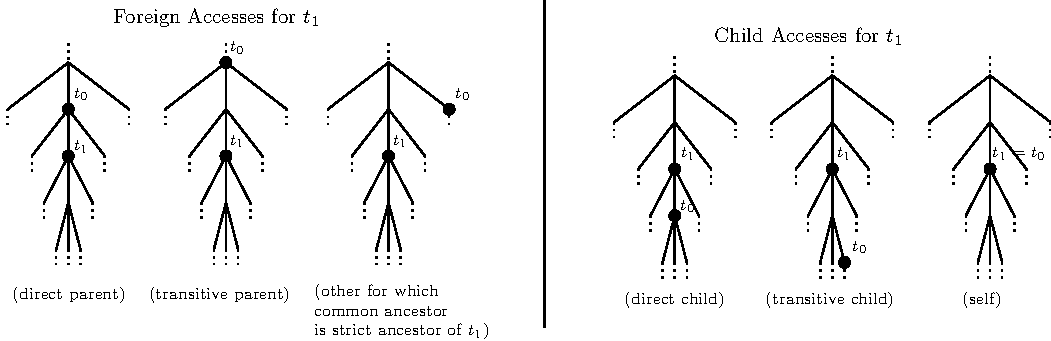
\includegraphics[width=\textwidth]{../figs/accesses-kinds.pdf}


\section{Tree Borrows implemented}

\subsection{Testing the Rust Standard Library}

\subsection{Performance concerns and optimizations}

Tree Borrows is slower than Stacked Borrows.

The semantics require that on every access, every tag of the allocation have its
permissions updated on the corresponding range. On allocations with many reborrows
this can easily lead to a naive implementation of Tree Borrows being slower than
Stacked Borrows by an arbitrarily large multiplicative factor.

Fortunately Tree Borrows has access to easy optimizations that allow it to have
an execution time in the same order of magnitude as that of Stacked Borrows on
realistic code samples. We observe that in practice the slowdown from Stacked Borrows
to Tree Borrows is mostly less than x2 on benchmarks that are specifically designed
to stress the borrow tracker, and about x1.3 on general tests that don't particularly attempt to
push the borrow tracker to its limits.


\begin{tabular}{|l|l|c|c|c|c|}
    \hline
    Project & Test & Runs & SB & TB & Factor \\
    \hline
    \multirow{2}{9em}{Miri}
        & \texttt{slice-get-unchecked} & 5 & 0.56s & 4.15s & {\color{Red}x7.41} \\
        & \texttt{mse} & 5 & 0.67s & 1.42s & {\color{Red}x2.12} \\
        & \texttt{serde1} & 5 & 1.53s & 2.60s & {\color{YellowOrange}x1.70} \\
        & \texttt{serde2} & 5 & 3.19s & 5.16s & {\color{YellowOrange}x1.62} \\
        & \texttt{unicode} & 5 & 1.27s & 1.99s & {\color{YellowOrange}x1.57} \\
        & \texttt{backtraces} & 5 & 4.01s & 5.81s & {\color{YellowOrange}x1.45} \\
    \hline
    \multirow{3}{9em}{Stdlib}
        & \texttt{core} & 1 & 4m31s & 9m15s & {\color{Red}x2.05} \\
        & \texttt{alloc} & 1 & 4m45s & 5m54s & {\color{LimeGreen}x1.24} \\
        & \texttt{std/time} & 1 & 15.1s & 17.5s & {\color{LimeGreen}x1.16} \\
    \hline
    \multirow{1}{9em}{Regex}
        & \texttt{lib} & 1 & 13.3s & 20.6s & {\color{YellowOrange}x1.54} \\
    \multirow{1}{9em}{Hashbrown}
        & \texttt{lib} & 1 & 31.5s & 38.3s & {\color{LimeGreen}x1.21} \\
    \multirow{1}{9em}{Tokio}
        & \texttt{lib} & 1 & 40.7s & 45.3s & {\color{LimeGreen}x1.11} \\
    \multirow{1}{9em}{Rand}
        & \texttt{lib} & 1 & 1m24s & 1m31s & {\color{LimeGreen}x1.08} \\
    \hline
\end{tabular}

\begin{itemize}
    \item Miri
        \begin{description}
            \item[Source] \href{https://github.com/rust-lang/miri}{\texttt{github:rust-lang/miri}}
            \item[Command] \texttt{MIRIFLAGS="" ./miri bench}
        \end{description}
    \item Miri-test-stdlib
        \begin{description}
            \item[Source] \href{https://github.com/rust-lang/miri-test-stdlib}{\texttt{github:rust-lang/miri-test-stdlib}}
            \item[Command] \texttt{MIRIFLAGS="" ./run-test.sh core --lib --tests}
            \item[Command] \texttt{MIRIFLAGS="" ./run-test.sh alloc --lib --tests}
            \item[Command] \texttt{MIRIFLAGS="-Zmiri-disable-isolation"}\\
                \texttt{./run-test.sh std --lib --tests -- time::}
        \end{description}
    \item Tokio
        \begin{description}
            \item[Source] \href{https://github.com/tokio-rs/tokio}{\texttt{github:tokio-rs/tokio}}
            \item[Command] \texttt{MIRIFLAGS="-Zmiri-disable-isolation -Zmiri-tag-raw-pointers"} \\
                \texttt{cargo +nightly miri test --features full --lib}
        \end{description}
    \item Rand
        \begin{description}
            \item[Source] \href{https://github.com/rust-random/rand}{\texttt{github:rust-random/rand}}
            \item[Command] \texttt{MIRIFLAGS="" cargo +nightly miri test --lib}
        \end{description}
    \item Hashbrown
        \begin{description}
            \item[Source] \href{https://github.com/rust-lang/hashbrown}{\texttt{github:rust-lang/hashbrown}}
            \item[Command] \texttt{MIRIFLAGS="" cargo +nightly miri test --lib}
        \end{description}
    \item Regex
        \begin{description}
            \item[Source] \href{https://github.com/rust-lang/regex}{\texttt{github:rust-lang/regex}}
            \item[Command] \texttt{MIRIFLAGS="" cargo +nightly miri test --lib -- --skip encode\_decode}
        \end{description}


\end{itemize}

\section{Future work}

\subsection{Formalization}

\subsection{Proving optimizations}


%%
%% Bibliography
%%
% Rustc dev guide: https://rustc-dev-guide.rust-lang.org/borrow_check/two_phase_borrows.html

\bibliography{literature}


\newpage
\appendix

\end{document}
